\hypertarget{Déroulement}{%
\chapter{Déroulement}\label{Déroulement}}

Ce chapitre, le plus volumineux du rapport, décrira l'ensemble des tâches que j'ai eu à effectuer au cours de ces trois semaines.

La première partie sera consacrée à la découverte théorique des réseaux de neurones artificiels classique, qui me permettra plus facilement de présenter les réseaux de neurones impulsionnels que j'ai implémenté.

\section{Théorie}
\subsection{Fonctionnement des réseaux de neurones}
La plupart de mes connaissances sur le sujet vient des présentations que nous ont faites les membres du groupe \textbf{SpikeTrain}, ainsi que d'un livre, co-écrit par le Pr. Paugam Moisy~\cite{naturalHandbook}.
En voici donc un rapide résumé.

\subsubsection{Neurone artificiel classique}
\label{neuroneClassique}
Tout d'abord avant de parler de réseaux de neurone à spike il serait de bon ton d'expliquer le principe du réseau de neurone classique, explication qui commencera par expliquer le
le principe du neurone unique.

Un neurone artificiel est pourvu d'un certain nombre d'\textbf{entrées}. Dans le cas des neurones classiques, ces entrées sont des nombres réels. Le neurone calculera, en fonction de ces entrées, une unique valeur en \textbf{sortie}.
Détaillons la façon dont ces calculs sont effectués:

Chacune de ces entrées circule sur une connection, laquelle est caractérisée par un \textbf{poids} qui définit l'importance de l'entrée pour le neurone.

Le neurone calcule dans un premier temps la somme de ses entrées, pondérée par leurs poids respectifs, à laquel vient s'ajouter un \textbf{biais} spécifique à chaque neurone (cf. equation~\ref{sommePonderee}).

\begin{equation}
\label{sommePonderee}
y = \sum_{i}^{n} w_i \times x_i + b
\end{equation}

Le résultat de cette somme passe alors dans une \textbf{fonction d'activation} qui permet d'introduire une non-linéarité dans les calculs. La sortie $s$ du neurone est donc calculée conformément à l'équation~\ref{calcNeurone}

\begin{equation}
\label{calcNeurone}
s = f(\sum_{s=0}^{n_{x}} x_{n}w_{n} + b)
\end{equation}

Un schéma reprenant ces explications est présenté dans la figure~\ref{neuroneSeul} :

\begin{figure}[h]
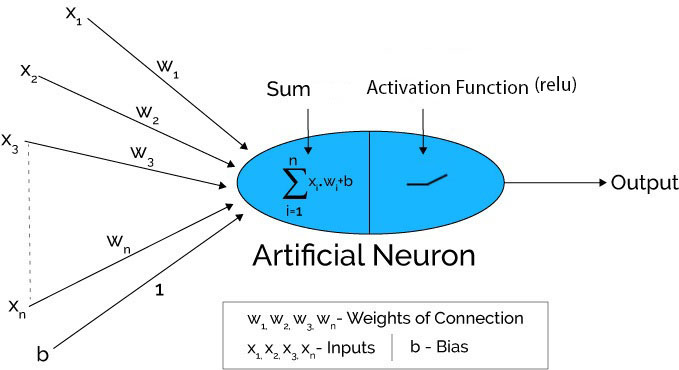
\includegraphics[width=16.5cm]{./images/image2.jpg}
\label{neuroneSeul}
\caption{Fonctionnement d'un neurone seul}
\end{figure}

Notre apprentissage ce fera en modifiant les poids de ses différentes
connexion (et le biais) de façon à obtenir une sortie proche de celle voulu.\newline

\subsubsection{Réseaux de neurones classiques}

Les neurones présentés précédemment prennent tout leur intérêt lorsqu'ils sont utilisés en groupes, dans des \textbf{réseaux de neurones}.

Le premier de ces réseaux, encore utilisé de nos jours, est appelé \textbf{perceptron}.
Le principe du perceptron n'est pas nouveau et date des années 1960.

Dans ces réseaux, les neurones sont organisés en \textbf{couches}.
La première couche correspond à celle qui permettra d'introduire des informations dans le réseau (comme la rétine par exemple). Elle est nommé \textbf{couche d'entrée}
La dernière couche permettra de lire les décisions du réseau. Elle est appelée \textbf{couche de sortie}. Dans les applications classiques, à chaque neurone de la couche de sortie correspond une décision possible et le neurone qui est le plus activé sur la couche de sortie l'emporte.
Entre ces couches, on trouve souvent un nombre variable de couches intermédiaires appelées \textbf{couches cachées}.

Entre deux couches, on établit le plus souvent un schéma de connexion que nous pouvons qualifier de \textit{full connected}, c-a-d que chaque neurone d'une couche est connecté avec chaque neurone de la couche suivante.Nous allons encore une fois, pour le bien de ce rapport, ne pas épiloguer sur les autres types de connexions existantes.\newline

Nous allons, pour cette partie encore, utiliser une figure (\ref{reseauClassique}) pour illustrer nos propos:

\begin{figure}[h]
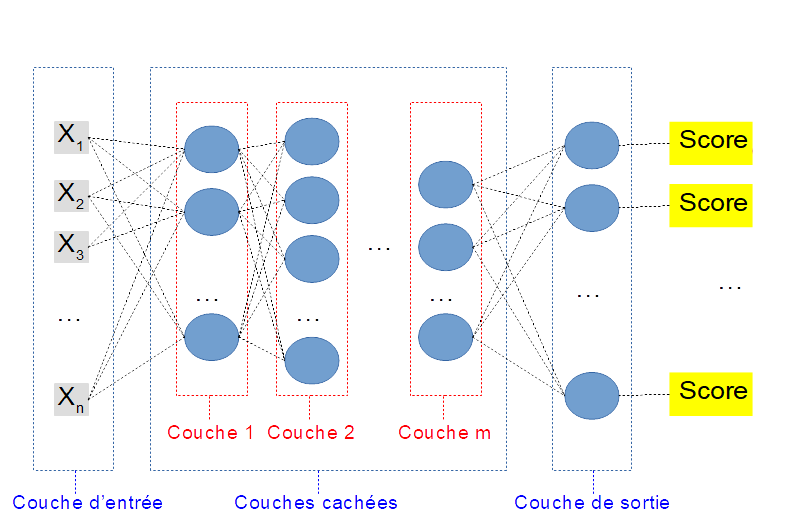
\includegraphics[width=16.5cm]{./images/multicouche.png}
\caption{réseau de neurones classique en couches}
\label{reseauClassique}
\end{figure}

Voyons maintenant en quoi les réseaux de neurones impulsionnels se distingue de ces neurones classiques.

\subsection{Réseaux de neurones impulsionnels}
\label{SNN}

Nous allons à présent aborder les neurones à Spikes aussi appelés réseaux de neurones impulsionnel. comme pour les réseaux de neurones classiques, nous allons expliquer le fonctionnement d'un neurone avant de détailler le fonctionnement d'un réseau de neurone impulsionnel.

\textit{Remarque} : Pour le reste de ce rapport nous utiliserons les anglicismes \textit{Spiker} \footnote{Spiker: Émettre une impulsions},\textit{Spike}\footnote{Spike: l'Impulsion émise par un neurone}.
Ces anglicismes sont en effet couramment utilisés entre chercheurs.

\subsubsection{Neurone à Spikes}
\label{neuroneSpike}

Comme les neurones classiques vu en section~\ref{neuroneClassique}, un neurone impulsionnel présente des \textbf{entrées} pondérées par des \textbf{poids} et une \textbf{unique sortie}.

En revanche, de façon plus proche du fonctionnement biologique, les neurones n'échangent plus des chiffres mais des \textbf{impulsions} (ou \textbf{spikes}).

Tous les spikes ont des propriétés similaires et ne se distinguent que par leur instant d'émission. En conséquence, dans un réseau de neurones impulsionnels, l'information n'est portée que par le positionnement temporel des spikes.

\textit{En plus d'être éloignée de la réalité nous avons des calculs lourd et couteux qui sont éffectuer sur chaque neurone ce qui demande une assez grande puissace de calcul donc une quantité d'énergie proportionelle.}

Une propriété primordiale du neurone à spike est son \textbf{potentiel de membrane} qui représente l'excitation du neurone.
En l'absence d'entrées, ce potentiel a une valeur dite \textbf{de repos}.

Lorsque qu'un spike arrive au neurone, ce spike déclenche l'augmentation du potentiel de membrane, selon une \textbf{équation différentielle}~\footnote{variable en fonction des modèles de neurones utilisés}.

Chaque nouveau spike induit ainsi des augmentations du potentiel de membranes proportionnelles aux poids des connections sur lesquelles ils arrivent.

L'équation différentielle induit également qu'en l'absence de nouveau spike, le potentiel tendra à revenir au potentiel de repos.

Si le potentiel de membrane atteint un certain \textbf{seuil}, le neurone \textbf{émet un spike en sortie}~\footnote{Après avoir spiké, un neurone devient réfractaire pendant un laps de temps, c-a-d qu'il ignore ses spikes d'entrée.}

En conséquence, c'est bien la notion de temps qui détermine si l'on émet un spike ou non. Pour émettre un spike, un neurone doit recevoir un nombre de spike dans un interval de temps suffisament court  pour permettre à son potentiel de membrane d'atteindre le seuil déclenchant l'émission.

Mais une fois de plus une image vaut mieux que mille mots:\newline

\begin{figure}[h]
  \begin{center}
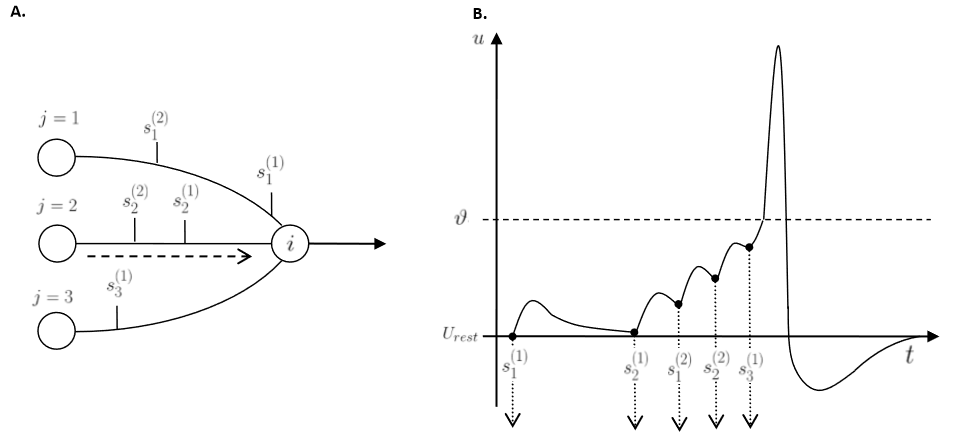
\includegraphics[width=12cm]{./images/image9.png}
\end{center}
\caption{Fonctionnement d'un neurone impulsionnel. \textbf{à gauche}~: le neurone $i$ reçoit des impulsions en provenance des entrées $j$ aux instants $s_k$. \textbf{à droite}~: évolution du potentiel de membrane du neurone $i$ en fonction du temps. Ce neurone émettra un spike peu après $s_3$}
\label{NeuroneASpike}
\end{figure}

\subsubsection{Reseau de neurones impulsionnels à reservoir}

Nous pouvons à présent attaquer les réseaux de neurones à spike.

Comme dans le cas des réseaux de neurones classiques, un réseau impulsionnel comporte le plus souvent une \textbf{couche d'entrée}, une \textbf{couche de sortie} et une \textbf{architecture intermédiaire} entre ces couches.

Le choix de cette architecture intermédiaire varie beaucoup plus que dans le cas des réseaux classiques. Durant ce stage, conformément à l'article de référence~\cite{Lympero} qui nous a guidés, nous utiliserons une architecture dite \textbf{de Reservoir Computing}, dans laquelle les couches ont disparues et les neurones sont simplement connectés les uns aux autres avec des connections récurrentes, formant un graphe.~\footnote{Pour les lecteurs plus forcenés, les autres architectures sont présentées en annexe.}

Comme pour chaque présentation, nous allons illustrer cette architecture par un exemple sur la figure~\ref{reservoir}

\begin{figure}[h]
  \begin{center}
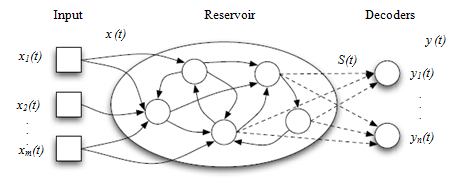
\includegraphics[width=8cm]{./images/Reservoir.png}
\end{center}
\caption{Architecture de reservoir computing}
\label{reservoir}
\end{figure}

Enfin, pour observer l'activité d'un réseau de neurones impulsionnel, on utilise une figure nommée \textbf{rasterplot}. Dans un rasterplot, l'axe des abscisses représente le temps et l'axe des ordonnées représente l'indice des neurones observés.
Un point dans un rasterplot tel que celui de la figure~\ref{principeRasterplot} représente un spike émis par un neurone donné, à un instant donné.

\begin{figure}[h]
  \begin{center}
  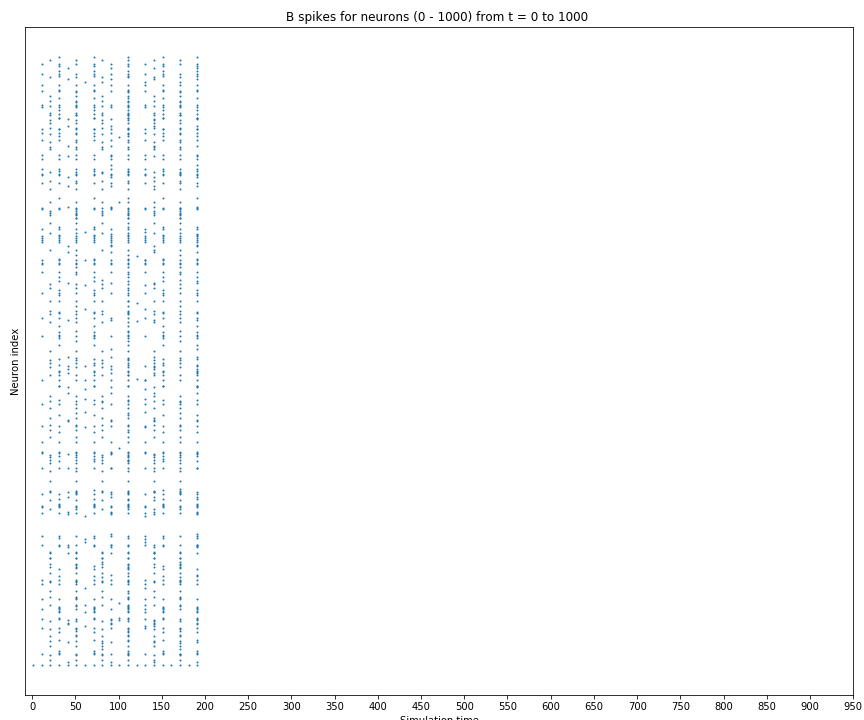
\includegraphics[width=8cm]{./images/SpikeB.png}
  \end{center}
  \caption{Exemple de rasterplot : On voit que les neurones émettent de façon relativement synchronisée avant de cesser brutalement.   }
  \label{principeRasterplot}
\end{figure}

\subsection{Le challenge}
\label{lechallenge}

Le challenge "Dyni Odontocete Click Classification, 10 species [ DOCC10 ]
by Universite de Toulon" (https://challengedata.ens.fr/challenges/32) consistait simplement à réaliser un classifieur qui classe les cachalots en une dizaine d'especes à partir de leurs "Clics" pour celà nous avions a disposition une base d'apprentissage labelisée ainsi qu'une base de test non labelisée sur laquelle nous pouvions évaluer les performances réelles de nos classifieurs. Pour cela nous labelision les exemples de la base de test puis envoyions nos prédictions sur le site du challenge qui nous renvoyais nos performances ainsi qu'un classement des performances de tous les participants.

Les deux bases sont consititués d'enregistrements audios des clics des différentes especes de cachalots que je présenterais plus en détail dans la partie analyse des données.

Pour résoudre ce probléme j'ai commencé par analyser les données afin
-D'avoir une vision claire du probléme a résoudre
-D'avoir des idées de méthodes de résolution du probléme
-Comprendre d'éventuelles incohérences dans nos futurs résultats (notament des différences de performances entre les deux bases)


Ensuite nous avons traité les données de différentes maniéres notament en faisant de la data augmentation et du traitement du signal.

Puis M. Clergue se chargeait de tester un multitude de techniques d'apprentissage sur les données ainsi traités.

M. Page nous a également fournis un grand nombre de petits programmes et de fonctions parfois simples parfois complexes dont nous avions besoin afin de réaliser nos différentes taches.

%\hypertarget{lechallenge}{%
\chapter{lechallenge}\label{lechallenge}}

Le challenge "Dyni Odontocete Click Classification, 10 species [ DOCC10 ]
by Universite de Toulon" (https://challengedata.ens.fr/challenges/32) consistait simplement à réaliser un classifieur qui classe les cachalots en une dizaine d'especes à partir de leurs "Clics" pour celà nous avions a disposition une base d'apprentissage labelisée ainsi qu'une base de test non labelisée sur laquelle nous pouvions évaluer les performances réelles de nos classifieurs. Pour cela nous labelision les exemples de la base de test puis envoyions nos prédictions sur le site du challenge qui nous renvoyais nos performances ainsi qu'un classement des performances de tous les participants.

Les deux bases sont consititués d'enregistrements audios des clics des différentes especes de cachalots que je présenterais plus en détail dans la partie analyse des données.

Pour résoudre ce probléme j'ai commencé par analyser les données afin
-D'avoir une vision claire du probléme a résoudre
-D'avoir des idées de méthodes de résolution du probléme
-Comprendre d'éventuelles incohérences dans nos futurs résultats (notament des différences de performances entre les deux bases)


Ensuite nous avons traité les données de différentes maniéres notament en faisant de la data augmentation et du traitement du signal.

Puis M. Clergue se chargeait de tester un multitude de techniques d'apprentissage sur les données ainsi traités.

M. Page nous a également fournis un grand nombre de petits programmes et de fonctions parfois simples parfois complexes dont nous avions besoin afin de réaliser nos différentes taches.


\section{le travail a distance}

\label{letravailadistance}

Comme vous le savez certainement durant cette année 2020 nous avons été touchés par la crise du coronavirus qui nous a conduit a être confinés nous forçant a travailler uniquement a distance.

Ces circonstances très particuliéres ont grandement affecté notre travail particulérement au début ou nous avons du régler de nombreux problémes techniques et organisationels. Cependant en nous forçant a nous adapter a ces nouvelles conditions, cette crise nous a permis de grandement augmenter nos competances en "télétravail".

Ainsi malgrés des débuts léthargiques nous avons mis en place une "routine de travail" qui était la suivante :
-Des visio-conférences quotidiennes nous permettant d'organiser et de synchroniser notre travail
-Un groupe whatsap dédié a mon stage afin de communiquer le plus efficacement possible
-Un Github privé dédié afin de partager l'ensemble du projet
-Un partage régulier de google collab via google drive

%\hypertarget{letravailadistance}{%
\chapter{letravailadistance}\label{letravailadistance}}

Comme vous le savez certainement durant cette année 2020 nous avons été touchés par la crise du coronavirus qui nous a conduit a être confinés nous forçant a travailler uniquement a distance.

Ces circonstances très particuliéres ont grandement affecté notre travail particulérement au début ou nous avons du régler de nombreux problémes techniques et organisationels. Cependant en nous forçant a nous adapter a ces nouvelles conditions, cette crise nous a permis de grandement augmenter nos competances en "télétravail".

Ainsi malgrés des débuts léthargiques nous avons mis en place une "routine de travail" qui était la suivante :
-Des visio-conférences quotidiennes nous permettant d'organiser et de synchroniser notre travail
-Un groupe whatsap dédié a mon stage afin de communiquer le plus efficacement possible
-Un Github privé dédié afin de partager l'ensemble du projet
-Un partage régulier de google collab via google drive


\subsection{Outils utilisés}

\subsection{Présentation de GitHub}

\begin{figure}[h]
  \begin{center}
  
\includegraphics[width=5cm]{./images/github.jpg}
  \end{center}
\end{figure}

Nous pouvons définir GitHub comme une plateforme de développement de projet in formatique en groupe. Elle s'implifie grandement le développement de projets. Elle permet de versioner ses programme et d'y apporter des modification en temps réel à plusieurs.

\subsubsection{Pourquoi Github}
Car celà permet une certaine synergie avec nos autres outils que nou verrons plus tard. Cette plateforme permet une facilité de développement de par sa fonctionnalité de versionnage de notre code à chaque changement ce qui permet une mise à jour dynamique ainsi que une relative facilitée a retourner à un état entérieur de notre programme ce qui permet une faciliter de débogage.Nous pouvons d'ailleur dire que ce rappport est entreposer sur Github et qu'il peut être récupérer facilement.Cette plateforme est aussi très connu dans le monde de la programmation ce qui sera utile pour notre future professionnel.

\subsection{Présentation de Google Colab}

\begin{figure}[h]
\begin{center}

\includegraphics[width=5cm]{./images/Colab_logo.png}
\end{center}
\end{figure}

Colab peut-être défini comme étant une plateforme d'éxécution pour notre code
il permet du fait que ce soit la puissance de calcul d'ordinateur géré par Google une vitesse d'exécution ainsi qu'une vitesse de téléchargement de base de données supérieur à celle qui nous est disponible en local.

\subsubsection{Pourquoi Colab}
En premier lieu pour la faciliter d'exéccution du code car ce n'est pas en local ce qui permet une exécution quasi immédiate du code sans aucune installation.Il est aussi facile de mettre sur github du code produit avec colab car c'est deux plateforme sont liées. Il permet de par l'utilisation du format Jupyter de mélanger code et texte (peu aussi comporter des images) dans notre notebook.

Voilà un exmple d'exécution avec colab:

\begin{figure}[h]
\begin{center}
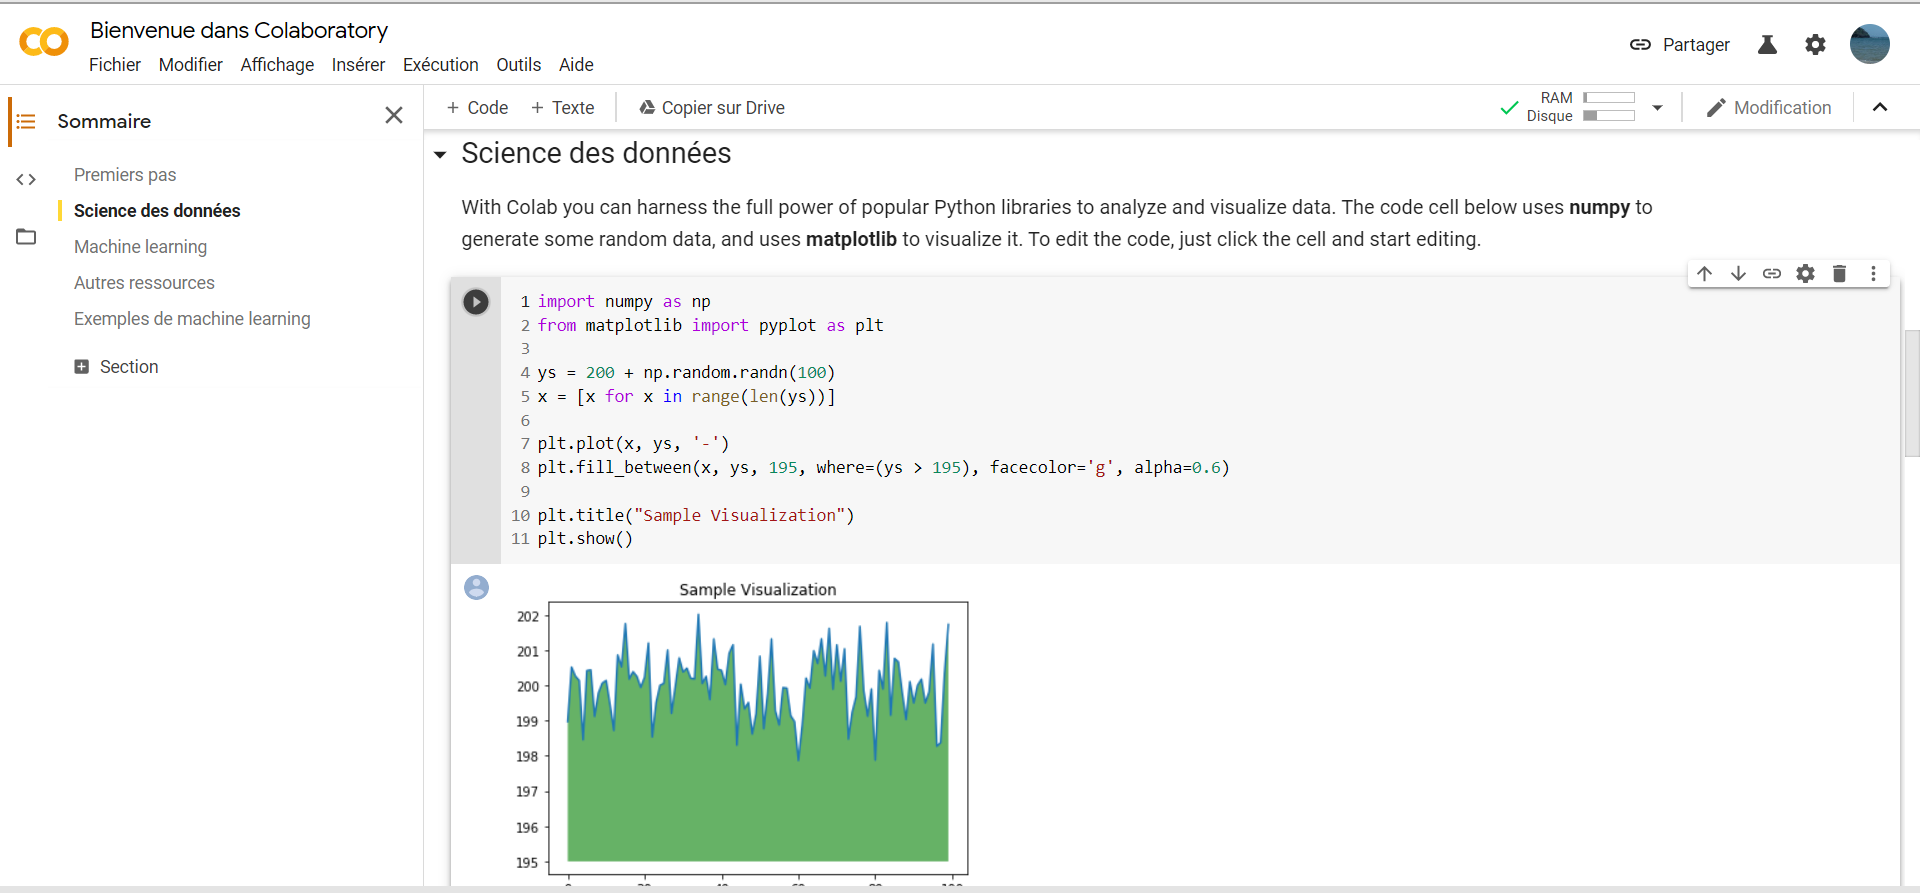
\includegraphics[width=15cm]{./images/Cap_colab.PNG}
\caption{Nous avons ici un exemple de code exécuté avec colab.}
\end{center}
\end{figure}


\subsection{Présentation de LaTex}

\begin{figure}[h]
  \begin{center}
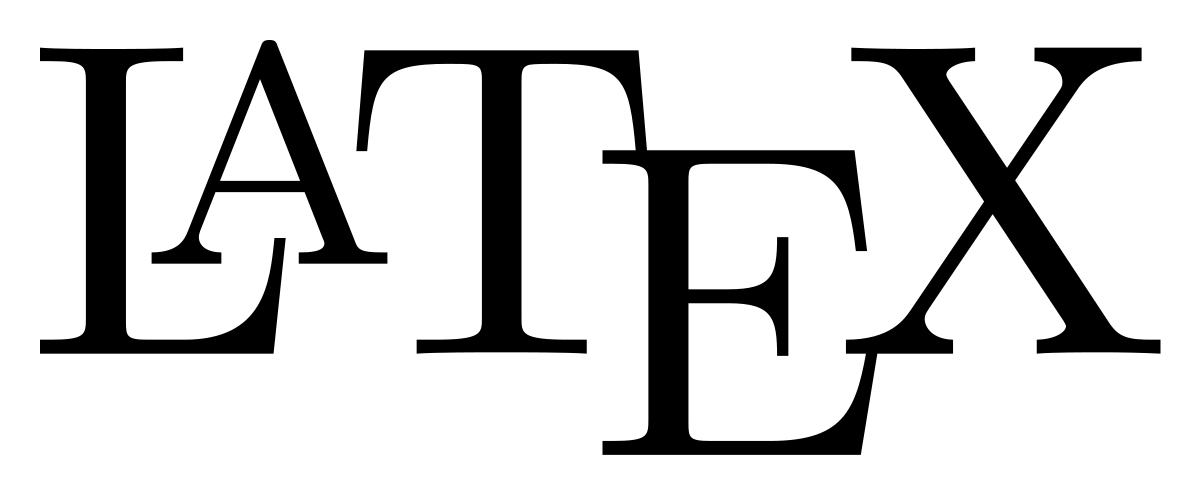
\includegraphics[width=5cm]{./images/Latex.png}
\end{center}
\end{figure}

Nous pouvons dire que LaTex est un langage de traitement de texte tel que le markdown qui permet de mettre en forme notre texte de manière \"scientifique\" cela veut dire que. LaTex permet une faciliter d'écriture des équations et de toutes les écriture mathématiques.Permet de par ses nombreux package une quasi-infinité de possibilitées.

\subsubsection{Pourquoi Github}
Cela permet encore une fois une synergie entre nos différent outil car LaTex peut-être utiliser avec un simple bloc-note c'est donc du texte ce qui permet une intéraction facilitée avec GitHub d'ailleurs ce rapport est écrit avec Latex et retrouvable sur GitHub.


%\subsection{Programme initial}



%\section{Premiers développements informatiques}
%\label{developpement}

%\subsection{Visualisation de la diffusion}
